\section{Introduction}
LLM agents rarely relies on a single model requests. Instead, they typically issue a series of dependent LLM calls to accomplish a task. Intermediate results evolve and stream across these calls as the agent executes, resulting in heavy KV-cache pressure. Agents' task performance is often bottlenecked by the efficiency of KV-cache management. Repeatedly processing and retaining these overlapping contexts
can impose substantial computation and memory overhead on the serving system. Efficient KV-cache management is therefore critical to improve the performance of serving LLM agents. Existing agent serving systems, such as Pythia \cite{yu2026pythia}, CacheScout~\cite{zhang2026cachescout}, PBKV ~\cite{zheng2026pbkv}, and KVFlow~\cite{pan2025kvflow}, optimize KV-cache management by exploiting future invocations and workflow information. They exploit these knowledge to guide KV-cache retention, eviction and prefetching. 

Meanwhile, agent frameworks increasingly expose LLM calls as programming abstractions rather than manual prompt construction. ByLLM~\cite{dantanarayana2025mtp} introduces a language-level abstraction that delegates function execution to an LLM, with the runtime using semantic information from the code like function signatures and parameter names to construct model requests. NVIDIA Object-Oriented Agents (NOOA)~\cite{furgale2026nooa} similarly embeds LLM-driven behavior into native Python objects and translates program-level declarations into prompts and model interactions. DSPy~\cite{khattab2024dspy} represents LM invocations through declarative signatures and modules, while the framework automatically generates a concrete prompt. This trend even extends beyond hand-written agent code. SIGIL~\cite{dantanarayana2026sigil} compiles natural-language skill documents into programs with explicit control flow and typed LLM calls, which the runtime lowers into prompts. Across these systems, LLM behaviors are specified using structured programming constructs, while framework runtimes translate those constructs into concrete prompts and model requests. 

These two trends expose an substantial granularity mismatch. Agent-serving systems optimize KV-cache management primarily at the granularity of requests and call sequences, whereas such LLM-as-programming-abstractions frameworks assemble each request from multiple program components. Therefore, treating such programmatically generated prompts as monolithic requests may lose valuable information for efficient LLM serving.

We observed that these programmatically generated LLM requests are inherently heterogeneous. Components within a generated prompt can have different sharing scopes and lifetimes. For example, some components may remain fixed across invocations, some are shared across call sites, and some can grow or be replaced as execution progresses. Figure~\ref{fig:heterogeneity-sample} shows an example, the four bindings of \texttt{assess\_evidence} have distinct lifetimes and evolution patterns. For example, \texttt{evidences} are session-scoped and accumulate over time, while \texttt{search\_results} is just a single-shot result. In this case, placing \texttt{evidences} after \texttt{search\_research} blocks KV-cache reuse of \texttt{evidences} across requests. Then model engine needs to recompute for these tokens, wasting scarce computational resource. This kind of differences in sharing scope and lifetime requires a more fine-grained management of KV-cache entries.

However, existing agent serving system are blind to this heterogeneity as they overlook the granularity inside the prompt. Mitigating this gap introduces two challenges. First, heterogeneity is not always explicit in the prompt, their sharing scope and lifetime are closely bonded with the program-level structure. Second, context scale and workflow evolution are often non-deterministic due to the inherent uncertainty of LLMs. Proactively management of KV-cache requires balance the trade-off between the cost of memory usage and the benefit of cache reuse. 


To close this gap, we propose \sysname, a compiler-server co-design that exploits prompt heterogeneity to achieve more efficient KV-cache management. \sysname's compiler pass performs static analysis to identify heterogeneous binding evolution patterns and application-level structure, and proactively re-layouts prompts to improve cache reuse. The serving runtime exploits the application-level structure and binding evolution patterns to optimize KV-cache behavior across requests by prefetching, protection, and eviction, according to the predicted future utility of cache entries. We implemented \sysname on SGLang~\cite{zheng2024sglang}. Our evaluation shows that \sysname ...

In summary, we make the following contributions.
\begin{itemize}
    \item We identify the inherent heterogeneity in programmatically generated prompts and its implications for serving.
    \item We design and build \sysname, a compiler-serving co-design that recovers and exploits prompt heterogeneity for efficient KV-cache management. 
    \item We conduct comprehensive evaluations of \sysname against multiple established serving systems, demonstrating that \sysname achieves up to...
\end{itemize}


\begin{figure}
    \centering
    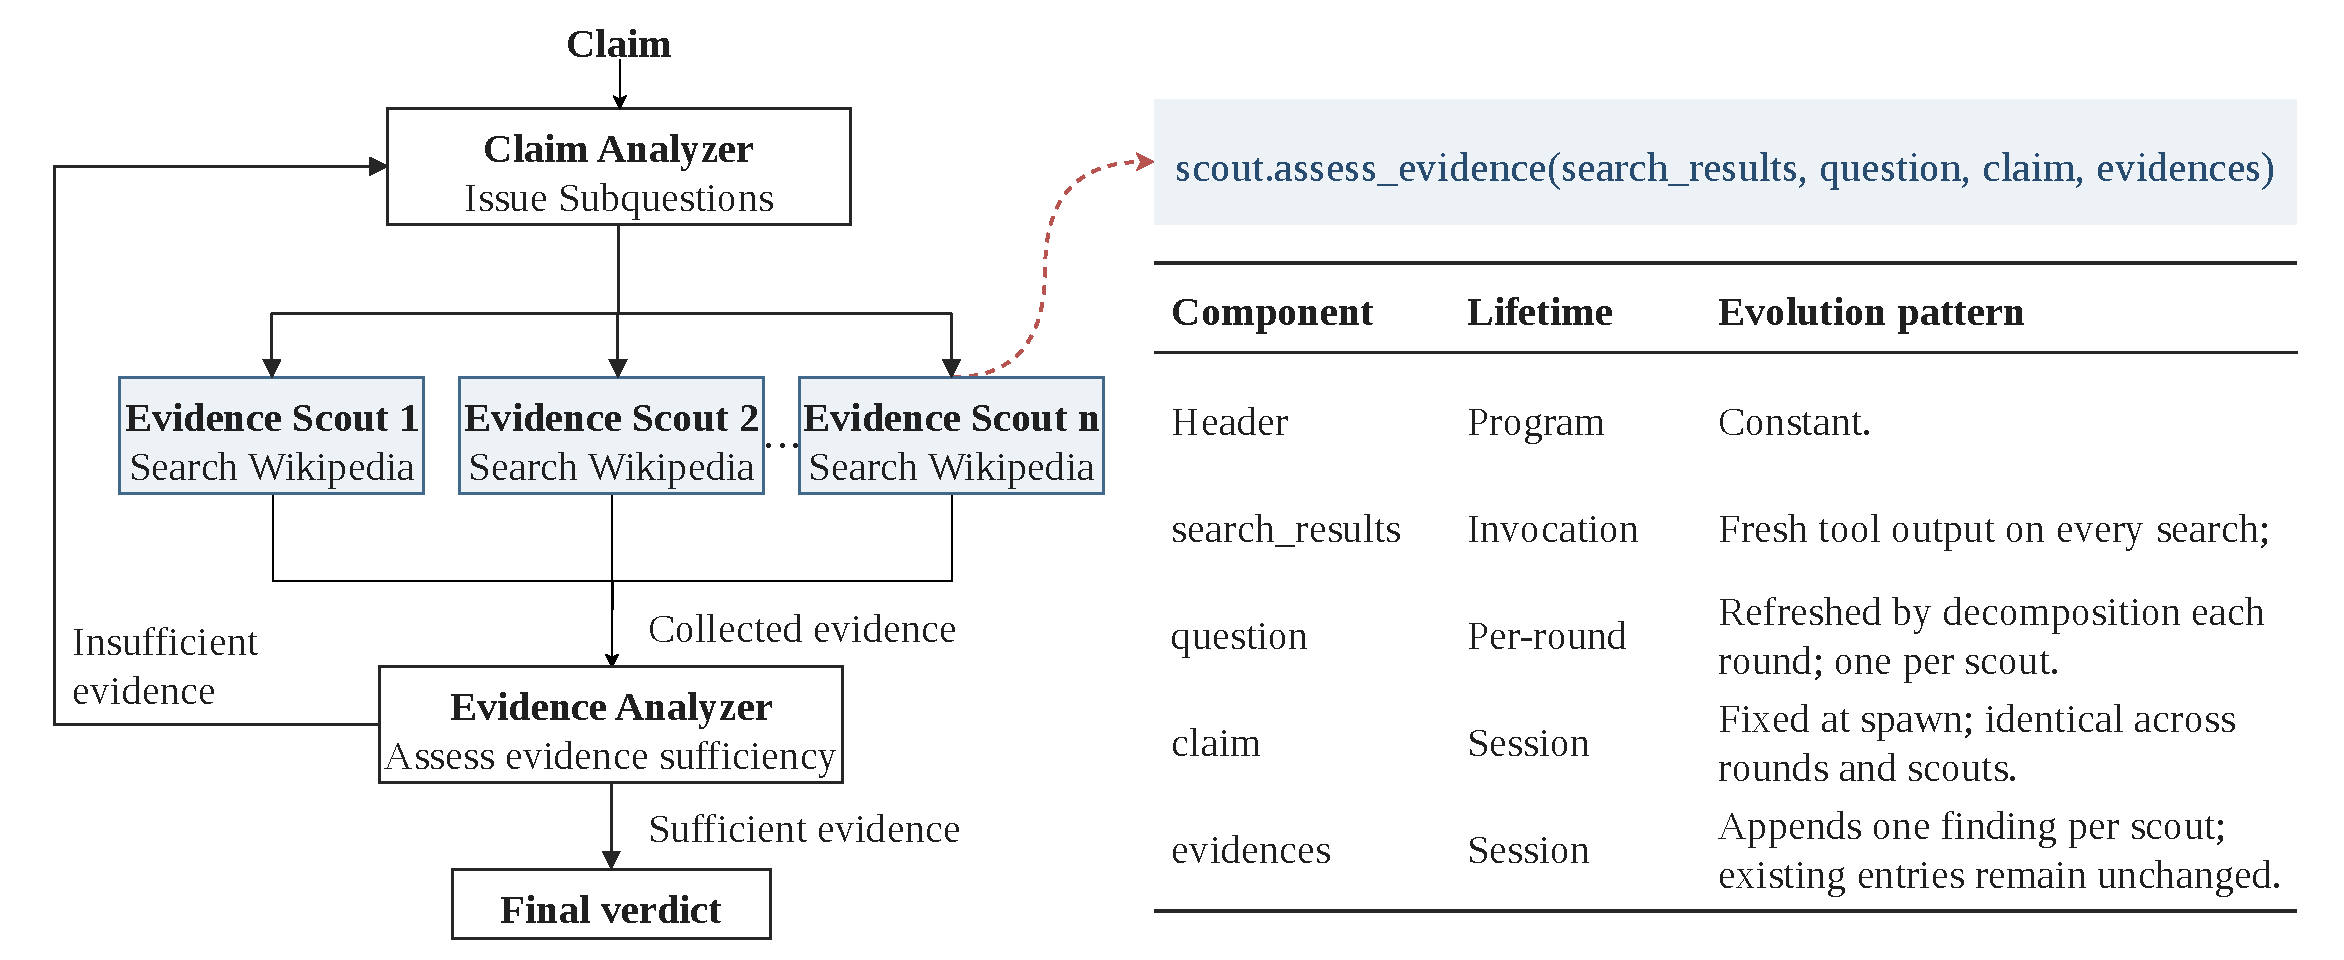
\includegraphics[width=1.0\linewidth]{figures/Sample_heterogeneity.pdf}
    \vspace{4pt}
    \begin{minipage}{\columnwidth}
    \ttfamily\footnotesize\raggedright
    def assess\_evidence(search\_results: str, question: str,\\   
    \hspace{12pt}claim: str, evidences: list[Evidence]) -> Finding by llm() \\
    \end{minipage}
    \caption{Heterogeneity within a HoVer-style \cite{jiang2020hover} Fact Check Agent's generated prompt for the summary-making function. \texttt{assess\_evidence(search\_results, question, claim, evidences)} evaluates the sub-question against the accumulated evidence and search results, then answers it.}
    \label{fig:heterogeneity-sample}
\end{figure}
